\documentclass[11pt,letterpaper]{article}
\usepackage[lmargin=1in,rmargin=1in,bmargin=1in,tmargin=1in]{geometry}
\usepackage{style/quiz}
\usepackage{style/commands}

% -------------------
% Content
% -------------------
\begin{document}
\thispagestyle{title}

% Quiz 1
\quizsol \textit{True/False}: If $P$ is the statement, ``$1 < 0$,'' and $Q$ is the statement, ``$1 + 1= 3$,'' then $P \to Q$ is false. \pspace

\sol The statement is \textit{false}. We define statements $P \colon 1 < 0$ and $Q \colon 1 + 1= 3$. We need to determine the truth value for $P \to Q$. Obviously, $1 \not< 0$, so $P$ is false. Furthermore, $1 + 1 \neq 3$, so that $Q$ is also false. So we know $P \equiv F_0$ and $Q \equiv F_0$. Therefore, $P \to Q$ is equivalent to $F_0 \to F_0$. Recall the truth table for $A \to B$:
	\begin{table}[h]
	\centering
	\begin{tabular}{c|c||c}
	$A$ & $B$ & $A \to B$ \\ \hline
	$T$ & $T$ & $T$ \\
	$T$ & $F$ & $F$ \\
	$F$ & $T$ & $T$ \\
	$F$ & $F$ & $T$
	\end{tabular}
	\end{table}
But then $P \to Q \equiv F_0 \to F_0$ is true. In fact, $A \to B$ is \textit{always} true if $A$ is false. Therefore, $P \to Q$ is true so that the statement of the quiz is false. \pvspace{1.3cm}



% Quiz 2
\quizsol \textit{True/False}: The circuit for $(P \wedge \neg Q) \vee \neg P$ is\dots
	\begin{figure}[h]
	\centering
	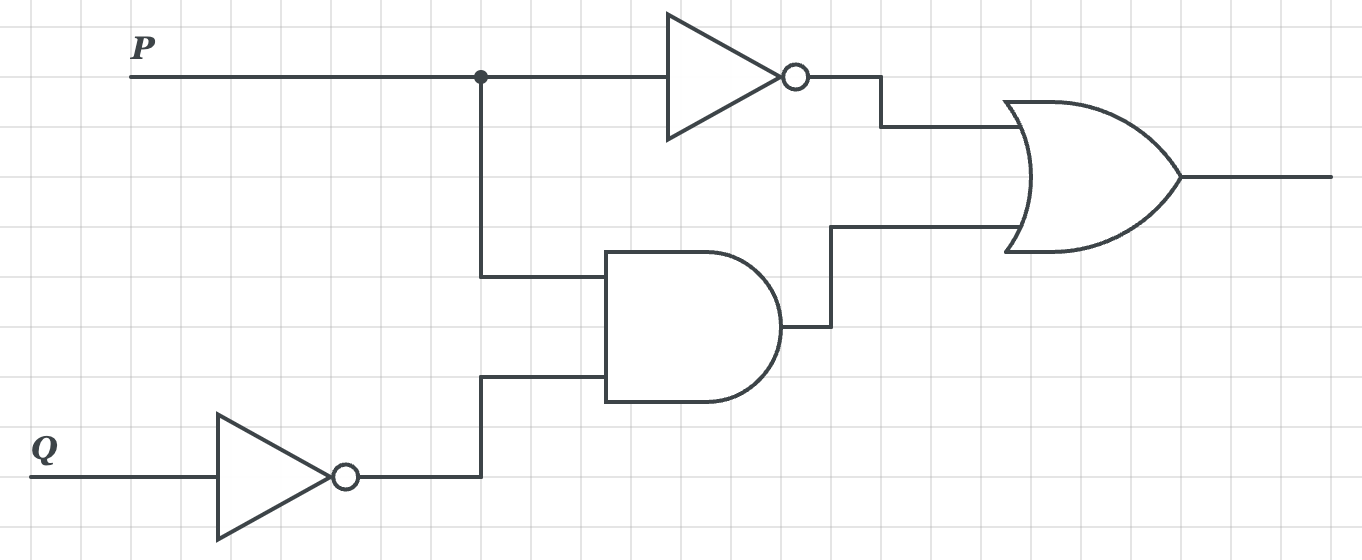
\includegraphics[width=0.5\textwidth]{images/qcircuit}
	\end{figure}


\sol The statement is \textit{true}. Following order of operations in $(P \wedge \neg Q) \vee \neg P$, we first compute $\neg Q$. As a circuit, we can represent $\neg Q$ as\dots
	\begin{figure}[H]
	\centering
	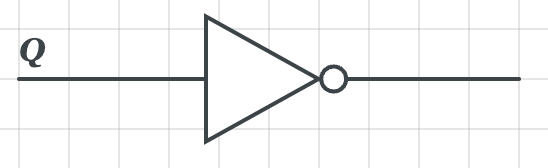
\includegraphics[width=0.25\textwidth]{images/negq}
	\end{figure}
We then `$\wedge$' (`and') this with $P$, which as a circuit is\dots
	\begin{figure}[H]
	\centering
	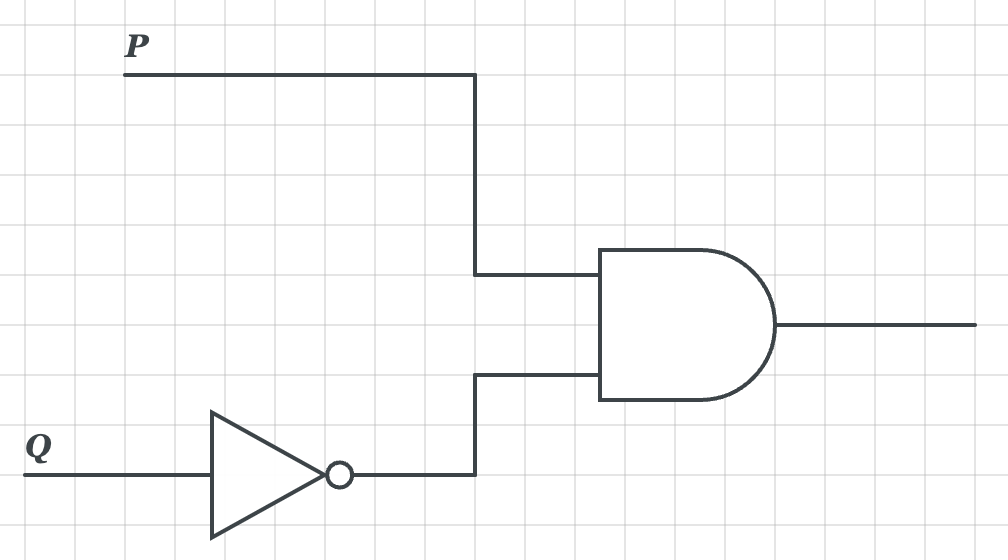
\includegraphics[width=0.3\textwidth]{images/negqand}
	\end{figure}
We then compute $\neg P$, which placing this in the circuit above, is\dots
	\begin{figure}[H]
	\centering
	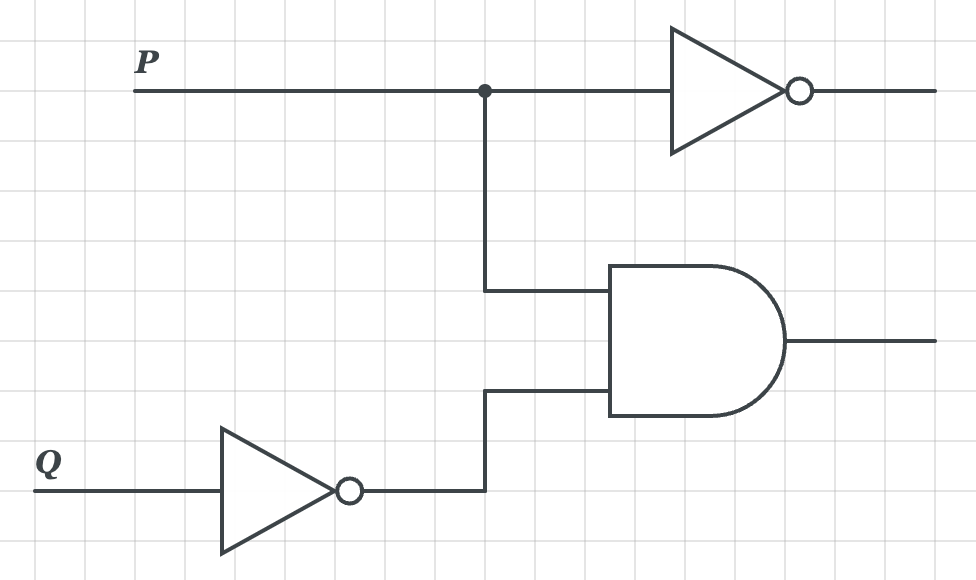
\includegraphics[width=0.3\textwidth]{images/negqandnegp}
	\end{figure}
We then `$\vee$' (`or') these outputs together, which yields\dots
	\begin{figure}[H]
	\centering
	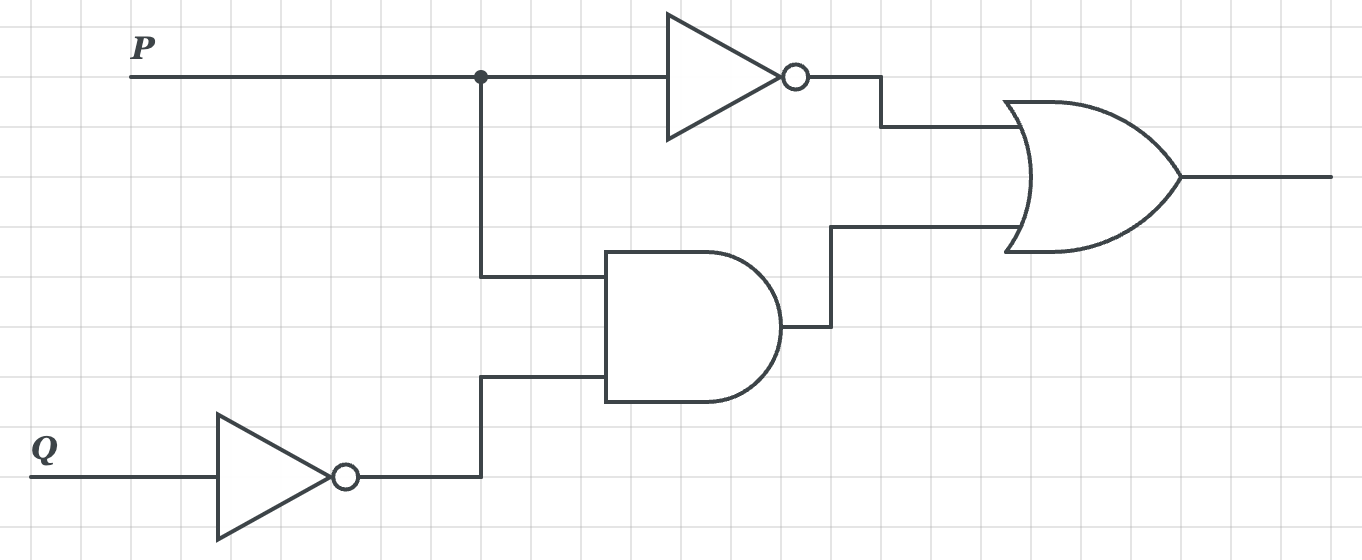
\includegraphics[width=0.5\textwidth]{images/qcircuit}
	\end{figure}
This is precisely the circuit given in the statement of the quiz. \pvspace{1.3cm}



% Quiz 3
\quizsol \textit{True/False}: XXXXVI is 46 in Roman numerals. \pspace

\sol The statement is \textit{false}. Recall that only certain symbols may be repeated sequentially in Roman numerals. For instance, $L$ and $D$ may \textit{not} be repeated sequentially. Furthermore, the repeatable sequentially symbols $I$, $X$, and $C$ may not be sequentially repeated more three times. In the quiz statement, $X$ is repeated sequentially four times. Therefore, this is not a valid Roman numeral. Clearly, the quiz statement of $X\!X\!X\!X\!V\!I$ is attempting to represent $X + X + X + X + V + I= 10 + 10 + 10 + 10 + 5 + 1= 46$. Because we cannot repeat $X$ four times in a row, rather than add up to $46$, we should count down to 46. Starting at 50, i.e. $L$, we need to subtract 10, which is $X$. Because we need to subtract this from $L$, we place it before $L$; that is, 40 is represented in Romain numerals by $X\!L$. We then add 6 to this resulting 40 to reach 46. We know 6 in Roman numerals is $V\!I$. Therefore, 46 in Roman numerals is $X\!LV\!I$. The statement of the quiz is then false. \pvspace{1.3cm}



% Quiz 4
\quizsol \textit{True/False}: Assuming perfect play, the first player wins the following NIM game:
	\[
	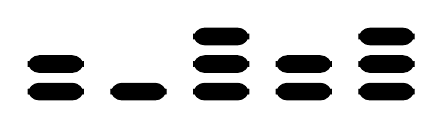
\begin{tikzpicture}[scale=0.7]
	% First Pile
	\draw[rounded corners,fill=black] (0,0) rectangle (1,0.3);
	\draw[rounded corners,fill=black] (0,0.5) rectangle (1,0.8);
	% Second Pile
	\draw[rounded corners,fill=black] (1.5,0) rectangle (2.5,0.3);
	% Third Pile
	\draw[rounded corners,fill=black] (3,0) rectangle (4,0.3);
	\draw[rounded corners,fill=black] (3,0.5) rectangle (4,0.8);
	\draw[rounded corners,fill=black] (3,1) rectangle (4,1.3);	
	% Fourth Pile
	\draw[rounded corners,fill=black] (4.5,0) rectangle (5.5,0.3);
	\draw[rounded corners,fill=black] (4.5,0.5) rectangle (5.5,0.8);	
	% Fifth Pile
	\draw[rounded corners,fill=black] (6,0) rectangle (7,0.3);
	\draw[rounded corners,fill=black] (6,0.5) rectangle (7,0.8);
	\draw[rounded corners,fill=black] (6,1) rectangle (7,1.3);	
	\end{tikzpicture}
	\]

\sol The statement \textit{true}. One method of determining this the `traditional' method. First, we count the number of chips in each heap:
	\[
	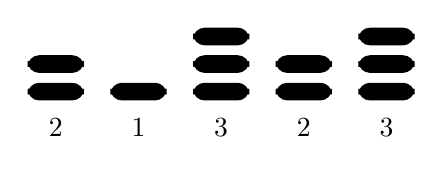
\begin{tikzpicture}[scale=0.7]
	% First Pile
	\draw[rounded corners,fill=black] (0,0) rectangle (1,0.3);
	\draw[rounded corners,fill=black] (0,0.5) rectangle (1,0.8);
	\node at (0.5,-0.5) {$2$};
	% Second Pile
	\draw[rounded corners,fill=black] (1.5,0) rectangle (2.5,0.3);
	\node at (2,-0.5) {$1$};
	% Third Pile
	\draw[rounded corners,fill=black] (3,0) rectangle (4,0.3);
	\draw[rounded corners,fill=black] (3,0.5) rectangle (4,0.8);
	\draw[rounded corners,fill=black] (3,1) rectangle (4,1.3);	
	\node at (3.5,-0.5) {$3$};
	% Fourth Pile
	\draw[rounded corners,fill=black] (4.5,0) rectangle (5.5,0.3);
	\draw[rounded corners,fill=black] (4.5,0.5) rectangle (5.5,0.8);	
	\node at (5,-0.5) {$2$};
	% Fifth Pile
	\draw[rounded corners,fill=black] (6,0) rectangle (7,0.3);
	\draw[rounded corners,fill=black] (6,0.5) rectangle (7,0.8);
	\draw[rounded corners,fill=black] (6,1) rectangle (7,1.3);	
	\node at (6.5,-0.5) {$3$};
	\end{tikzpicture}
	\]
We the number of chips in each heap in binary:
	\[
	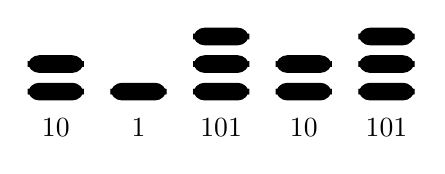
\begin{tikzpicture}[scale=0.7]
	% First Pile
	\draw[rounded corners,fill=black] (0,0) rectangle (1,0.3);
	\draw[rounded corners,fill=black] (0,0.5) rectangle (1,0.8);
	\node at (0.5,-0.5) {$10$};
	% Second Pile
	\draw[rounded corners,fill=black] (1.5,0) rectangle (2.5,0.3);
	\node at (2,-0.5) {$1$};
	% Third Pile
	\draw[rounded corners,fill=black] (3,0) rectangle (4,0.3);
	\draw[rounded corners,fill=black] (3,0.5) rectangle (4,0.8);
	\draw[rounded corners,fill=black] (3,1) rectangle (4,1.3);	
	\node at (3.5,-0.5) {$101$};
	% Fourth Pile
	\draw[rounded corners,fill=black] (4.5,0) rectangle (5.5,0.3);
	\draw[rounded corners,fill=black] (4.5,0.5) rectangle (5.5,0.8);	
	\node at (5,-0.5) {$10$};
	% Fifth Pile
	\draw[rounded corners,fill=black] (6,0) rectangle (7,0.3);
	\draw[rounded corners,fill=black] (6,0.5) rectangle (7,0.8);
	\draw[rounded corners,fill=black] (6,1) rectangle (7,1.3);	
	\node at (6.5,-0.5) {$101$};
	\end{tikzpicture}
	\]
We can then find the NIM sum:
	\begin{table}[h]
	\centering
	\begin{tabular}{rrr}
	0 & 1 & 0 \\
	0 & 0 & 1 \\
	1 & 0 & 1 \\
	0 & 1 & 0 \\
	1 & 0 & 1 \\ \hline
	0 & 0 & 1
	\end{tabular}
	\end{table}
Because the NIM sum is not 0, we know that this is an $N$-position. Therefore, the current player, i.e. the \textit{\underline{N}}ext to move, is the winner---assuming perfect play. Furthermore, we can determine the winning move from the NIM sum. The next player needs to make the NIM sum zero. Observe that one winning move would be to remove the heap of one as then the NIM sum would be zero. One could also remove one chip from either heap of three---resulting in a total of three heaps of size two. These are the only winning moves. Alternatively, one can recall that in traditional NIM, one can ignore matching heaps. We have matching heaps of size two and three. Ignoring these, we only have a heap of size one. It is then clear that the NIM sum is not zero and this NIM game is equivalent to a game with a single heap of size one. It is also then obvious that a winning move is to remove the heap of size one. Finally, recall also that in traditional NIM, one can ignore chips (in any heap) in matching pairs of size 1, 2, 4, 8, \dots. Observe that we can find two matching pairs of chips of size two and two matching chips of size one. This would leave only one remaining chip. This again forces this to be an $N$-position with a winning move to be to remove the heap of size one. In any case, assuming perfect play, the first player wins the given NIM game. \pvspace{1.3cm}



% Quiz 5
\quizsol \textit{True/False}: If you take out a simple discount note for 6~months for \$1,400 and receive \$1,156, the interest you pay is \$244. \pspace

\sol The statement is \textit{true}. The interest paid is the discount on the note. The amount you receive from the loan is the loan amount minus this discount. The loan was for \$1,400 and you received \$1,1156. Therefore, you paid $\$1400 - \$1156= \$244$ in interest. We can also compute this directly. We know that the discount (interest) paid on a loan is given by $D= Mrt$, where $D$ is the discount, $M$ is the maturity (the loan amount), $r$ is the yearly interest rate, and $t$ is the loan length (in years). The amount you receive, $L$, is the maturity minus the discount, i.e. $L= M - D= M - Mrt= M( 1 - rt)$. We know that $M= \$1400$, $L= \$1156$, and $t= \frac{6}{12}= 0.50$. Therefore, we have\dots
	\[
	\begin{aligned}
	L&= M(1 - rt) \\
	\$1156&= \$1400 (1 - 0.50r) \\
	\dfrac{\$1156}{\$1400}&= \dfrac{\$1400 (1 - 0.50r)}{\$1400} \\
	0.825714&= 1 - 0.50 r \\
	-0.174286&= -0.50 r \\
	\dfrac{-0.174286}{-0.50}&= \dfrac{-0.50 r}{-0.50} \\
	r&= 0.348572
	\end{aligned}
	\]
But then we have $D= Mrt= \$1400 \cdot 0.348572 \cdot 0.50 \approx \$244$, as given in the quiz statement. \pvspace{1.3cm}



% Quiz 6
\quizsol \textit{True/False}: If you deposit \$8,000 in an account earning 5\% annual interest, compounded quarterly, the amount in the account after 6~years is $8000 \left(1 + \frac{0.50}{4} \right)^6$. \pspace

\sol The statement is \textit{false}. We know that if a principal, $P$, is invested at an annual interest rate, $r$, compounded $k$ times per year, is invested for $t$ years that the amount, $F$, it will be worth is given by $F= P \left(1 + \frac{r}{k} \right)^{kt}$. We know that $P= \$8000$ and $r= 0.05$. Because the interest is compounded quarterly, i.e. every fourth of a year, the interest is compounded four times per year, i.e. $k= 4$. Finally, we know $t= 6$. Therefore, we would have\dots
	\[
	\begin{aligned}
	F&= P \left(1 + \frac{r}{k} \right)^{kt} \\
	&= \$8000 \left(1 + \frac{0.05}{4} \right)^{4 \cdot 6} \\
	&= \$8000 (1.0125)^{24} \\
	&\approx \$8000 (1.34735105) \\
	&\approx10778.81	
	\end{aligned}
	\]
Observe that the expression in the statement of the quiz, i.e. $8000 \left(1 + \frac{0.50}{4} \right)^6$, an interest rate of $0.50$ is used rather than a rate of $0.05$. Furthermore, the exponent is 6, the number of years, rather than $24= 4 \cdot 6$, the number of compounds. If one computes the expression given in the quiz, an amount of \$16,218.29 is obtained. Therefore, the quiz statement is \textit{false}. \pvspace{1.3cm}



% Quiz 7
\quizsol \textit{True/False}: If $\vec{u}= \langle 1, 0, -3 \rangle$ and $\vec{v}= \langle 2, 5, 1 \rangle$, then $\vec{u} \cdot \vec{v}= \langle 2, 0, -3 \rangle$. \pspace

\sol The statement is \textit{false}. There is no `traditional multiplication' for vectors; that is, there is no `multiplication' for vectors that has all the `usual' properties. We are asked to compute the dot product of two vectors. The dot product always results in a scalar, i.e. a number. The given result is a vector. Therefore, the quiz statement is false. The result given is the simple component-wise product of the two vectors.  Recall that the dot product of two vectors $\vec{a}, \vec{b}$, is given by $\vec{a} \cdot \vec{b}= \sum a_i b_i$; that is, the dot product of two vectors is the sum of the product of the corresponding components for the vectors. Therefore, we have\dots
	\[
	\vec{u} \cdot \vec{v}= \langle 1, 0, -3 \rangle \cdot \langle 2, 5, 1 \rangle= 1(2) + 0(5) + (-3)1= 2 + 0 - 3= -1
	\]
Furthermore, because $\vec{u} \cdot \vec{v} \neq 0$, we know that the given vectors are not perpendicular. Finally, because $\vec{u} \cdot \vec{v} < 0$, we know that vectors point in `opposite' directions, i.e. that the angle between them is greater than $90^\circ$. \pvspace{1.0cm}



% Quiz 8
\quizsol \textit{True/False}: If $\vec{u}$ and $\vec{v}$ are vectors, then $\text{proj}_{\vec{v}}\, \vec{u}= \dfrac{\vec{v} \cdot \vec{u}}{\vec{v} \cdot \vec{v}}$. \pspace

\sol The statement is \textit{false}. We know that $\text{proj}_{\vec{v}}\, \vec{u}$ is a vector---the vector that represents `how much' of $\vec{u}$ points `in the direction' of $\vec{v}$. In particular, $\text{proj}_{\vec{v}}\, \vec{u}$ is a vector that is parallel or antiparallel to $\vec{v}$. Observe that $\dfrac{\vec{v} \cdot \vec{u}}{\vec{v} \cdot \vec{v}}$ is a scalar, i.e. a number, because $\vec{v} \cdot \vec{u}$ and $\vec{v} \cdot \vec{v}$ are numbers. However, this scalar is the magnitude of amount needed to scale/reflect $\vec{v}$ to be $\text{proj}_{\vec{v}}\, \vec{u}$. We should have\dots
	\[
	\text{proj}_{\vec{v}}\, \vec{u}= \left( \dfrac{\vec{v} \cdot \vec{u}}{\vec{v} \cdot \vec{v}} \right) \vec{v}=  \left( \dfrac{\vec{v} \cdot \vec{u}}{\| \vec{v} \|^2} \right) \vec{v}= \left( \dfrac{\vec{v} \cdot \vec{u}}{\| \vec{v} \|} \right) \dfrac{\vec{v}}{\|\vec{v}\|}
	\] \pvspace{0.8cm}



% Quiz 9
\quizsol \textit{True/False}: If $A$ and $B$ are matrices, then $AB= BA$. \pspace

\sol The statement is \textit{false}. While ordinary multiplication for real numbers is commutative, e.g. $2 \cdot 3= 3 \cdot 2$, this is \textit{not} generally true for matrices. For instance, let us take $A= \begin{pmatrix} 1 & 1 \\ 0 & 2 \end{pmatrix}$ and $B= \begin{pmatrix} 0 & 2 \\ 3 & 1 \end{pmatrix}$. Then we have\dots
	\[
	\begin{aligned}
	AB&= \begin{pmatrix} 1 & 1 \\ 0 & 2 \end{pmatrix} \begin{pmatrix} 0 & 2 \\ 3 & 1 \end{pmatrix}= \begin{pmatrix} 1(0) + 1(3) & 1(2) + 1(1) \\ 0(0) + 2(3) & 0(2) + 2(1) \end{pmatrix}= \begin{pmatrix} 0 + 3 & 2 + 1 \\ 0 + 6 & 0 + 2 \end{pmatrix}= \begin{pmatrix} 3 & 3 \\ 6 & 2 \end{pmatrix} \\[0.3cm]
	BA&= \begin{pmatrix} 0 & 2 \\ 3 & 1 \end{pmatrix} \begin{pmatrix} 1 & 1 \\ 0 & 2 \end{pmatrix}= \begin{pmatrix} 0(1) + 2(0) & 0(1) + 2(2) \\ 3(1) + 1(0) & 3(1) + 1(2) \end{pmatrix}= \begin{pmatrix} 0 + 0 & 0 + 4 \\ 3 + 0 & 3 + 2 \end{pmatrix}= \begin{pmatrix} 0 & 4 \\ 3 & 5 \end{pmatrix}
	\end{aligned}
	\] 
But then we see that $AB \neq BA$. While there may be specific matrices $A, B$ where $AB= BA$, it is not generally true that $AB= BA$ for matrices. \pvspace{1.1cm}



% Quiz 10
\quizsol \textit{True/False}: If $A= \begin{pmatrix} 2 & -6 \\ 1 & -3 \end{pmatrix}$, then $A^{-1}$ exists. \pspace

\sol The statement if \textit{false}. We know that for square matrices $M$, $M^{-1}$ exists if and only if $\det M \neq 0$. Recall that for two-by-two matrices $M$, say $M= \begin{pmatrix} a & b \\ c & d \end{pmatrix}$, that $\det M= ad - bc$. But then we have\dots
	\[
	\det A= \det \begin{pmatrix} 2 & -6 \\ 1 & -3 \end{pmatrix}= 2(-3) - (-6)1= -6 - (-6)= 0
	\]
But because $\det A= 0$, we know that $A^{-1}$ does not exist. \pvspace{1.3cm}



% Quiz 11
\quizsol \textit{True/False}: If you have $2x - 3y \leq 10$, you shade below the resulting line. \pspace

\sol The statement if \textit{false}. We know that the given inequality represents a line because this is a two-variable, linear inequality. We first find the corresponding line. Solving for $y$, recalling that if we multiply or divide both sides of the inequality by a negative number we need reverse the `direction' of the inequality, we find\dots
	\[
	\begin{aligned}
	2x - 3y &\leq 10 \\
	-3y&\leq -2x + 10 \\
	\dfrac{-3y}{-3}&\geq \dfrac{-2x}{-3} + \dfrac{10}{-3} \\
	y&\geq \frac{2}{3}\, x - \frac{10}{3}
	\end{aligned}
	\]
Therefore, the line corresponding to the inequality $2x - 3y \leq 10$ is $y= \frac{2}{3}\,x - \frac{10}{3}$. We know that given a point $(x, y)$ in the plane, if $y= \frac{2}{3}\,x - \frac{10}{3}$, we are on the line. From the inequality above, we want $y$ to be at least as large as $\frac{2}{3}\,x - \frac{10}{3}$. So $y$ need `move up.' Therefore, we shade above the line $y= \frac{2}{3}\,x - \frac{10}{3}$. But then we shade above the line corresponding to $2x - 3y \leq 10$. \pvspace{1.3cm} 



% Quiz 12
\quizsol \textit{True/False}: Any graph with more than one edge is a multigraph. \pspace

\sol The statement is \textit{false}. A multigraph is a graph with multiple edges (or loops). However, this does \textit{not} mean that the graph has more than one edge. This means that the graph has two vertices with more than one edge connecting them. For instance, the graph $G$ on the left below is a multigraph, whereas the graph $H$ on the right below is \textit{not} a multigraph. 
	\[
	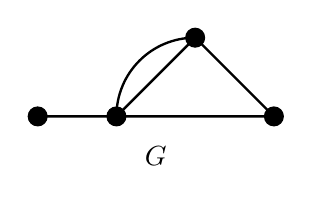
\begin{tikzpicture}
	\draw[line width=0.03cm] (0,0) -- (1,0) -- (2,1) -- (3,0) -- (1,0);
	\draw[line width=0.03cm] (1,0) to[out=90, in= 180] (2,1);
	
	\draw[fill=black] (0,0) circle (0.12);
	\draw[fill=black] (1,0) circle (0.12);
	\draw[fill=black] (2,1) circle (0.12);
	\draw[fill=black] (3,0) circle (0.12);
	
	\node at (1.5,-0.5) {$G$};
	\end{tikzpicture} \hspace{2cm}
	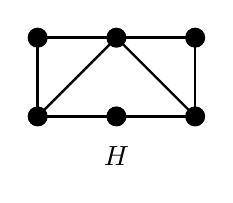
\begin{tikzpicture}
	\draw[line width=0.03cm] (0,0) -- (2,0) -- (2,1) -- (0,1) -- (0,0);
	\draw[line width=0.03cm] (0,0) -- (1,1) -- (2,0);
	
	\draw[fill=black] (0,0) circle (0.12);
	\draw[fill=black] (1,0) circle (0.12);
	\draw[fill=black] (2,0) circle (0.12);
	\draw[fill=black] (0,1) circle (0.12);
	\draw[fill=black] (1,1) circle (0.12);
	\draw[fill=black] (2,1) circle (0.12);
	
	\node at (1,-0.5) {$H$};
	\end{tikzpicture}
	\] \pvspace{1.3cm}



% Quiz 13
\quizsol \textit{True/False}: An Euler circuit cannot have a repeated vertex. \pspace

\sol The statement is \textit{false}. It is important to recall the definitions and differences between Euler and Hamiltonian circuits. Because each are circuits, they must begin and end at the same vertex. However, an Euler circuit visits every edge in the graph without repeating an edge. Vertices may be repeated for an Euler circuit. \textbf{E}uler circuits are about \textbf{E}dges. Hamiltonian circuits visit every vertex without repeating a vertex. So Euler circuits can repeat vertices but not edges. Hamiltonian circuits can repeat edges but not vertices. [Repeating an edge would always result in a repeated vertex.] \pvspace{1.3cm}



% Quiz 14
\quizsol \textit{True/False}: If a graph has adjacency matrix $A$ and 
	\[
	A^5= \begin{pmatrix} 0 & 14 & 18 \\ 14 & 16 & 12 \\ 18 & 12 & 0 \end{pmatrix}
	\]
then there are 16~walks from vertex two to itself. \pspace

\sol The statement is \textit{false}. Recall that the adjacency matrix $A$ is the the number of edges between pairs of vertices. That is, the matrix $A= (a_{ij})$ is the matrix where $a_{ij}$ is the number of edges from vertex $v_i$ to vertex $v_j$. Powers of the adjacency matrix gives different information about the graph. Suppose $A$ is the adjacency matrix of a graph and $P= A^n$ is the $n$th power of the adjacency matrix. If $P= (p_{ij})$, then $p_{ij}$ is the number of distinct walks of length $n$ from the vertex $v_i$ to the vertex $v_j$ in the graph. Because $A$ is adjacency matrix of the graph, we know the entries of $A^5$ give the number of walks of length five between specified vertices. If we want the number of walks of length five from $v_2$ to $v_2$, we want the entry $p_{2,2}$ of the matrix $P= A^5$. This is the entry in the second row and second column. While this is indeed 16, this is the number of walks of length five, specifically. The statement of the quiz is false because one must specific the length of the walk. There may be many more walks (of any length) from $v_2$ to $v_2$. There may be no such walks for specific lengths, e.g. there may be walks of length four from $v_2$ to $v_2$ but no walks of length three. \pvspace{1.3cm}



% Quiz 15
\quizsol \textit{True/False}: If $A$ has probability $0.40$ and $B$ has probability $0.50$, then $A$ or $B$ has probability $0.40 + 0.50= 0.90$. \pspace

\sol The statement is \textit{false}. To compute $P(A \text{ or }B)$, you cannot simply add the probabilities of $A$ and $B$ unless you know that $A$ and $B$ are disjoint. Otherwise, you may be overestimating the probability of $P(A \text{ or }B)$. All we know is that $0 \leq P(A \text{ or }B) \leq P(A) + P(B)$. To see an example where the quiz statement fails, suppose that $A$ is the event that a student received a 90 or greater on an exam and $B$ is the statement that a student received an 80 or greater on the exam. Then we know that 40\% of students received a 90 or higher on the exam and 50\% of students received a 80 or higher on the exam. The statement $A \text{ or } B$ is the statement that a student received a 90 or higher on the exam or received an 80 or higher on the exam. But this is just the event that a student received an 80 or higher on the exam. But then we know that $P(A \text{ or } B)= 0.50$ because we know that 50\% of students received an 80\% or higher. But $P(A) + P(B)= 0.40 + 0.50= 0.90$! What happened? We know that 40\% of students received a 90\% or higher on the exam. We know also that 50\% of students received an 80\% or higher on the exam. But the majority of that 50\% of students that received 80\% or higher were already accounted for by the 40\% of students that received a 90\% or higher. Thinking carefully, we see that 10\% of students received between an 80\% and 90\% on the exam. Simply adding $P(A)$ and $P(B)$ overestimates the probability by `double counting' those that received a 90\% or higher on the exam. Generally, we have $P(A \text{ or }B)= P(A) + P(B) - P(A \text{ and } B)$. Using this and the work above, we find $P(A \text{ or } B)= P(A) + P(B) - P(A \text{ and } B)= 0.40 + 0.50 - 0.40= 0.50$. \pvspace{1.3cm}



\newpage



% Quiz 16
\quizsol \textit{True/False}: If $A$ has probability $0.40$ and $B$ has probability $0.50$, then $A$ and $B$ has probability $0.40 \cdot 0.50= 0.20$. \pspace

\sol The statement is \textit{false}. To compute $P(A \text{ and } B)$, you cannot simply multiply $P(A)$ and $P(B)$ unless you know that the events $A, B$ are independent. That is, generally $P(A \text{ and } B) \neq P(A) \cdot P(B)$. This is because once $A$ or $B$ occurs, the probability of $B$ or $A$, respectively, occurring may change. For instance, suppose that $A$ is the event that you receive an `A' on an exam and $B$ is the event you receive a `$B$' on an exam. Because $P(A)= 0.40$ and $P(B)= 0.50$, there is a 40\% chance you receive an `A' on the exam and a 50\% you receive a `B' on the exam. Now $P(A) \cdot P(B)= 0.40 \cdot 0.50= 0.20$ but we know $P(A \text{ and } B)= 0$ because you cannot receive \textit{both} a `A' and `B' on the exam simultaneously---you receive one or the other or neither. Generally, we know that $P(A \text{ and } B)= P(A) \cdot P(B \;|\; A)$, where $P(B \;|\; A)$ is the conditional probability that $B$ occurs, assuming that $A$ occurs. We can resolve this issue above because we know you cannot receive a `B' if you receive an `A'. Therefore, $P(A \text{ and } B)= P(A) \cdot P(B \;|\; A)= 0.40 \cdot 0= 0$, as expected. \pvspace{1.3cm}



% Quiz 17
\quizsol \textit{True/False}: The IQR of a dataset measures the spread about the median. \pspace

\sol The statement is \textit{true}. We know that $\text{IQR}= Q_3 - Q_1$, where $Q_3$ is the third quartile and $Q_1$ is the first quartile. The median is the `middle' of the data, i.e. $Q_2$. We know that $Q_1 \leq Q_2 \leq Q_3$. But then $\text{IQR}= Q_3 - Q_1$ gives the distance from $Q_1$ to $Q_3$, i.e. the spread about $Q_2$, which is the median. \pvspace{1.3cm}



% Quiz 18
\quizsol \textit{True/False}: Suppose $x$ is a random value from a normal distribution. Then the larger $|z_x|$ is the more `unusual' the value of $x$ is. \pspace

\sol The statement is \textit{true}. We know that $z_x$ measures the number of standard deviations $x$ is above/below the mean. We know also that the further $x$ is from the mean in a normal distribution, the more `unusual' $x$ is. But then the more positive or more negative $z_x$ is, i.e. the larger the value of $|z_x|$, the more `unusual' $x$ is. Recall that $z_x= \frac{x - \mu}{\sigma}$, where $\mu$ is the mean and $\sigma$ is the standard deviation. We know that $x - \mu$ is the distance from $x$ to $\mu$. If $x - \mu < 0$, then $x < \mu$; if $x - \mu > 0$, then $x > \mu$, and if $x - \mu= 0$, then $x= \mu$. But then $\frac{x - \mu}{\sigma}$ is the number of standard deviations $x$ is from $\mu$. We know that if $z_x < 0$, then $x$ is below the mean; if $z_x > 0$, then $x$ is above the mean, and if $z_x= 0$, then $x= \mu$. \pvspace{1.3cm}



% Quiz 19
\quizsol \textit{True/False}: The binomial distribution is used to find probabilities of counts that satisfy certain conditions. \pspace

\sol The statement is \textit{true}. The binomial distribution gives the probability that an event occurs a certain number of times out of a fixed number of trials. For instance, a binomial distribution can be used to find the probability of a certain number of heads if you flipped a coin ten times. The assumptions that need to be met for the binomial distribution to apply are\dots
	\begin{itemize}
	\item There are a fixed number of trials/observations, $n$.
	\item There are only two possible outcomes for each trial/observation. 
	\item The probability of each outcome is fixed, i.e. constant, throughout the trials/observations.
	\item The trials/observations are independent. 
	\end{itemize}
For instance, the number of heads obtained when flipping a coin ten times is a binomial distribution: there is a fixed number of trials (the ten coin flips), there are only two possible outcomes for each trial (heads or tails), the probability of each outcome is fixed (the probability is 50\% for heads and 50\% for tails during each flip), and the trials are independent (getting a head/tail on a particular flip does not `affect' the probability of obtaining a head/tail on the next flip). \pvspace{1.3cm}



% Quiz 20
\quizsol \textit{True/False}: Under certain conditions, the normal distribution can be used to approximate probabilities for the binomial distribution. \pspace

\sol The statement is \textit{true}. For instance, plotting the probability of obtaining $k= 1, 2, 3, \ldots, 40$ heads if one flips a coin 40 times, we obtain the following plot: \par
	\begin{figure}[h]
	\centering
	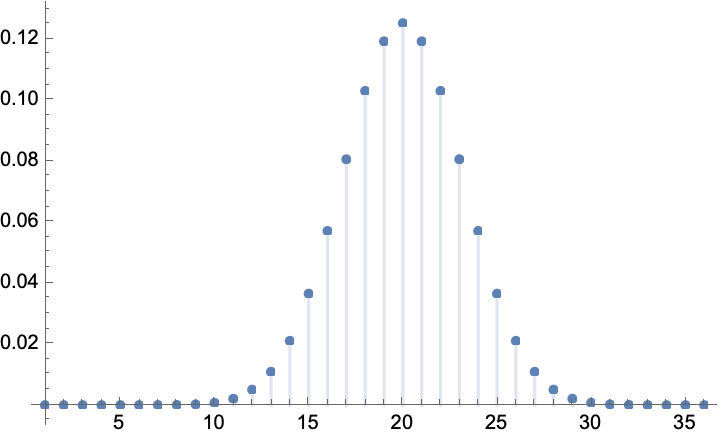
\includegraphics[width=0.4\textwidth]{images/binomplot.png}
	\end{figure} \par
We know that this process is binomial. Observe that this distribution is approximately normal. In fact, this will generally be the case for binomial distributions with `sufficiently large' $n$---that the distribution is approximately normal. This (non-obviously) follows from the Central Limit Theorem. If you have a binomial distribution $B(n, p)$ and $n$ is `sufficiently large' (for instance, $np \geq 10$ and $n(1 - p) \geq 10$), then we know that $B(n, p) \approx N \left(np, \sqrt{np(1 - p)} \right)$. That is, the binomial distribution is approximately a normal distribution with mean $\mu= np$ and standard deviation $\sigma= \sqrt{np(1 - p)}$.  


\end{document}